\chapter{Lufträume, Verkehr und Teamflug}\label{cha:airspace}\index{Luftraum}\index{FLARM}\index{Teamflug}

Es stehen eine Menge an Luftraumdatenbanken und Geländefiles als \menulabel{\bmenut{Konfig.}{2/3}\blink\bmenus{System}}  OpenSource zur Verfügung. Die
jeweils aktuellen Luftraumdaten für Deutschland können direct vom DAEC heruntergeladen und sofort
benutzt werden.: 
\begin{center}
  \url{http://www.daec.de/fachbereiche/luftraum-flugbetrieb/luftraumdaten/}
 \end{center}\menulabel{\bmenus{Standortdatei}\blink\bmenus{Standortdatei}}
 Neben den stets aktuellen Lufträumen stehen dort auch Sprungzonen und die Grenze Deutschlands zum Download. 
 
 Es können zwei Luftraumdateien \button{Lufträume} und \button{weitere Lufträume}in den Konfigurationseinstellungen benannt und benutzt werden, welche auch beliebig bearbeitet werden können. Benutzt wird hierbei das \textsf{OpenAir}-Format.\index{Luftraum!Dateiformat}



Es obliegt allein dem Benutzer, daß die jeweilige Datenbank aktuell ist.

Mi einem angeschlossenen Flarm, kann \xc  auch Luftverkehr anzeigen (natürlich nur von solchen
Luftfahrzeugen, die ebenfalls mit Flarm ausgestattet sind)

Es ist eine TeamCode Funktion implementiert, die es gestattet, die Partner farblich auf dem Display zu
markieren und über einen kurzen von \xc verschlüsselten FunkCode die exakte Position zu übermitteln.


\section{Anzeige der Lufträume}

Spezielle, lokale Lufträume werden mit einem dicken Rahmen versehen
als schattierter Bereich dargestellt. Die Farbe und die Schattierungen der
Flächen kann individuell konfiguriert werden.

Abhängig von den jeweiligen Einstellungen kann der Benutzer alle,
nur die Lufräume unter, die Lufträume unterhalb einer einzugebenden Höhe oder
aber Lufträume in einem bestimmten Höhenband angezeigt bekommen.


\begin{center}
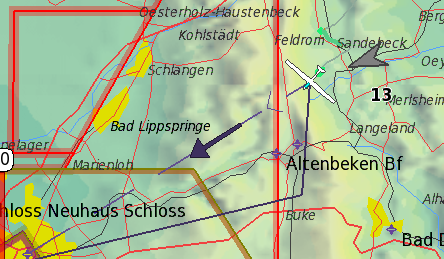
\includegraphics[angle=0,width=0.8\linewidth,keepaspectratio='true']{figures/airspace.png}
\end{center}

Zur Kennzeichnung der Lufträume werden diverse Stiloptionen wie Transparenz, Farben,
Schattierungen, und Linienoptionen bereitgestellt. 

Die nicht-transparenten  Darstellungen erlauben ein Durchscheinen von
Geländemerkmalen und Topologie, jedoch \emph{kein} Durchscheinen anderer Lufträume!
Wenn jedoch überlappende Lufträume auftreten sollten, werden die Grenzen der
Lufträume grundsätzlich angezeigt, egal, ob der Luftraum transparent oder nicht angelegt wurde.

Sowohl die Luftraumwarnungen als auch die Luftraumdarstellungen können individuell editiert werden,
hierzu siehe Kap.~\ref{sec:airsp-filt-dial}.

Die Standard Darstellung und Einfärbung der lufträume ist analog den aktuellen ICAO Karten

\section{Luftraumverletzungs Ereignisse}

Es werden drei Ereignisse in Bezug auf eine evtl. Luftraumverletzung  registriert und verarbeitet:
%Three types of events are detected by XCSoar in relation to SUA:
\begin{description}
\item[Wahrscheinliche Verletzung] Dies Ereignis wird registriert
wenn das Flugzeug bei Beibehalten des Kurses, der Geschwindigkeit und der Höhe in Kürze in einen Luftraum einfliegen wird.
Die Zeit der Vorhersage kann unter "Luftraum Warnung" in den Konfigurationseinstellungen eingestellt werde\index{Luftraumwarnung!Dauer bis Eintritt}

Da hier ein recht langer ermittelter und zukünftig angenommener Kurs des Flugzeuges als
 Grundlage benutzt wird, erlaubt \xc rechtzeitige Warnungen auch dann, wenn dies z.B.\
 durch Windabdrift beim Kurbeln erfolgen sollte.
\item[Eintreten] Dies Ereignis wird registriert beim Eintritt des Luftfahrzeuges in den Luftraum.
\item[Verlassen] Dies Ereignis wird registriert beim Verlassen des Luftfahrzeuges aus dem Luftraum.
\end{description}
Die Lufträume werden in allen Fällen bestimmt durch die Koordinaten sowie obere und
untere Höhe, wie diese im Luftraum-File eingetragen sind.

Luftraum, Warnungen werden ebenfalls ausgegeben, sollte sich bspw.\ durch einen zu großen Zoom-Level
 die  Grenze des Luftraumes außerhalb des aktuellen Kartenauschnittes befinden !
off-screen.

Wenn die barometrische Höhe vorhanden ist und dem System zugeführt werden kann, wird diese auf
jeden Fall der GPS Höhe vorgezogen und zu Berechnungen herangezogen.
Neben besserer Genauigkeit macht dies das System konform zum QNH-basierten System der
Flugflächen und Lufträume.

\section{Levels der Luftraumwarnungen}\label{airspace-level}

Erläuterung der Level der Lufaumwarnungen:
\begin{description}
\item[0] Luftfahrzeug ist außerhalb und entfernt vom Luftraum.
\item[1] Ein Eintreten in den Luftraum wird vorhergesagt, aber das Luftfahrzeug ist nicht nahe dran.
\item[2] Ein Eintreten in den Luftraum wird vorhergesagt und ist kurz davor, dies zu tun.
\item[3] Luftfahrzeug ist innerhalb des Luftraumes.
\end{description}

Über die gesamte Laufzeit zeichnet \xc die Postion des Luftfahrzeuges  relativ zu den
Lufträumen auf und generiert Warn-level für jeden Luftraum.

Die entsprechenden Warnungen werden kontinuierlich gemäß der Einstellungen
Filter gefiltert, sodaß entsprechende "ungefährliche" Lufträume effektiv ausgeblendet
 werden können.

Eine Annäherung mit anschließendem Eintreten in einen Luftraum führt führen typischerweise zu drei Warnungen :
Wenn in der Nähe $\rightarrow$ level 1, wenn dicht dran $\rightarrow$ level 2, wenn drinnen, $\rightarrow$ level 3

Wann immer der Warnlevel über 0 steigt (für jeden Luftraum) wird eine
Luftraumwarnung ausgegeben und ein Benachrichtigungston für Altair und PDA erfolgt.
Wenn keine weiteren Lufträume in der Nähe sind, welche oberhalb level 0 sind,
wird der Dialog automatisch geschlossen.


\section{Luftraumwarnungs-Dialog}

Der Luftraumwarnung-Dialog beinhaltet eine Liste von bis zu 4 individuellen  Warnungen.
Der Hintergund der Listeneintrage ist \textcolor[rgb]{0.97,0.17,0.19}{\textbf{rot}}, wenn das Flugzeug
sich im Luftraum befindet, und gelb, wenn das Flugzeug nahe ist.

Wenn die Warnung bestätigt wurde, wird der Text der Warnung ausgegraut.

Jede Liste beinhaltet zwei Spalten  und diese enthalten die folgenden Details:



\begin{verbatim}
<NAME>                <TOP>   <Inside>
<distance if outside> <BASE>
\end{verbatim}

Diese Werte werden kontinuierlich aktualisiert.

Éin Beispiel:

\begin{verbatim}
Bern TMA Class D     FL100     near
dist 1300                 1750m
\end{verbatim}

Dies bedeutet, daß das Flugzeug 1300m horizontal
entfernt vom Luftraum D 'Bern TMA'  ist die untere Grenze liegt bei
1750m und die obere grenze ist Flugfläche 100



Ein weiteres Beispiel:
\begin{verbatim}
Bern CTRgld Class C 1350m	    inside
                    SFC
\end{verbatim}

Das bedeutet, daß sich das Flugzeug im Luftraum C ''Bern CTRgld'' befindet,
dessen Untergrenze der Boden und obere Grenze 1300m ist.

Informationen  zu Lufträumen und  bzw.\  Luftraumwarnungen  können zu jeder
Zeit  über das Menü:

\bmenus{Info}\blink\bmenut{Was ist}{hier?}\index{Was ist hier?}\blink\bmenus{Details}

abgerufen werden.

Die Luftraumwarnungen werden solange wiederholt, solange man sich
nicht deutlich weit genug von scharfgeschalteten Lufträumen entfernt befindet.

\section{Luftraumwarnung-Bestätigung}

Wenn eine Luftraumwarnung angezeigt wird und der entsprechende
Luftraum aktiv ist, kann diese Warnung durch ''Schließen''  geschlossen werden.
Hiermit kann das Fenster ohne eine Bestätigung geschlossen werden.

Sollten eine oder mehrere Luftraumwarnungen sichtbar sein, so kann jede einzelne von diesen durch einen entsprechenden Button am unteren Ende bestätigt werden. (Hier ist Paderborn-TMZ blau hinterlegt, also zur Bearbeitung angewählt) 

\sketch{figures/airspacewarning_2.png} Die Anwahl des entsprechenden Luftraumes geschieht beim Altair mit dem Drehknopf, beim PDA mit dem Cursor.

Die einzelnen Bedeutungen der Bestätigungen sind wie folgt:

\begin{description}
%\item[\button{Warnung Bestätigen}] Bestätigung des Warn-Levels. Nur dann,
%wenn sich der Warn-Level \textsl{erhöht} (s. Kap. \ref{airspace-level}) erscheint
%eine neue Warnung entsprechend des neuen Levels.

\item[\button{Best. Luftraum}]  Bestätigt alle Warnungen für diesen Luftraum mit einem
innerhalb eines horizontalen Abstandes von 2500m und vertikal 500m.
Werden diese  Grenzen unterschritten, erscheint erneut eine Warnung.$\Rightarrow$  (F6 Taste on Altair)

\item[\button{Best. Tag}]  Alle laufenden und zukünftigen Warnungen für diesen Luftraum
und für den restlichen Flug werden unterdrückt und als bestätigt angenommen.
Das gilt solange, bis \xc bzw. Altair  wieder neu gestartet wurde, oder aber der
Luftraum explizit wieder aktiviert wurde (s.u.). $\Rightarrow$  (F7 Taste on Altair)

\item[\button{Schließen}] Schließt das Luftraumwarnungsfenster ohne jede Bestätigung.
Die Warnungen werden entsprechend wiederholt.
\end{description}

Einmal bestätigte Lufträume können  wieder zur Warnung aktiviert werden.  Siehe auch im folgenden Kapitel. \ref{sec:air-ack}
\index{Luftraumwarnung!Aktivieren}\index{Luftraumwarnung!Bestätigen}

\menulabel{\bmenut{Info}{3/3}\blink\bmenus{Lufträume}} Bitte beachtet, daß nicht alle Bestätigungs-Buttons bei allen Warnungen erscheinen!
Speziell, wenn man sich \textsl{innerhalb} eines Luftraumes befindet, gibt es keine Option
zur Bestätigung, denn der Warnmechanismus hat keine Veranlassung vor einer \textsl{bevorstehenden} Luftraumverletzung zu warnen.

Ihr seid ja bereits drin!!!

Generell sollte man mit den Luftraumwarnungen wie folgt umgehen:
\begin{itemize}
\item Bestätige keine Warnung, wenn Du vorhast, diesen Lufraum zu vermeiden!
\item Der Warton ertönt lediglich, wenn der Alarm\textsl{level} ansteigt.
\item Das Warnsystem ist so ausgelegt, daß es das Kurbeln neben einem Luftraum erlaubt,
ohne den Piloten extrem zu "nerven" Lediglich wenn es wirklich eng wird, werden
deutliche Warnungen wieder aktiviert\dots
\end{itemize}

Wenn ein Luftraum als "bestätigt" markiert wurde, wird dieser Luftraum
ohne farbliche Rahmen und Schraffur dargestellt.

Wenn ein Eindringen in einen Luftraum vorhergesagt wird oder aber ein
Eintreten bereits erfolgt, wird ein Warnfenster mit einer Meldung des Typs
des Luftraumes, der Unter- und Obergrenze (Höhe über Grund oder aber
Flugfläche) sowie der Frequenz des Luftraumes.
Begleitet wird dies von einem Warnton.


%\begin{center}
%\includegraphics[angle=0,width=0.7\linewidth,keepaspectratio='true']
%\end{center}

Bestätigte Lufträume werden nach einer festgelegten Zeit, der "Bestätigungszeit"
\menulabel{\bmenut{Konfig.}{2/3}\blink\bmenus{System}}wieder angezeigt und in die Alarmfunktion integriert. 

Diese Zeit kann in den Konfigurationseinstellungen unter \button{Bestätigungszeit} festgelegt werden

\menulabel{\button{Kartenanzeige}\blink\button{Luftraum}} 
Alle Luftraumwarnungen werden für jeden einzelnen Luftraum ausgegeben, das heißt,
 wenn z.B.\ das Flugzeug in einen Luftraum \textsf{A} einfliegt und kurze
Zeit später in einen \textsl{darin}liegenden Luftraum \textsf{B}, dann wird
nach der Meldung für \textsf{A} ebenfalls eine Warnung für den Luftraum
\textsf{B} zusätzlich erscheinen.

\tip Wenn gewünscht ist, daß die Warnungen nicht wiederholt werden, setze die
 Bestätigungszeit auf einen sehr großen Wert (z.B. 30min)\dots
 \index{Luftraumwarnung!Bestätigungszeit}

Die Luftraumwarnungen werden automatisch zurückgenommen, sobald die
Flugzeugposition \emph{und}  der angenommene zukünftige Kurs nicht auf einen
demnächst potentiell zu treffenden Luftraum zeigt.

Es kann zu gleichzeitigen  Luftraumwarnungen kommen, wenn  das Flugzeug
(oder der angenommene zukünftige Kurs) mehrere Lufträume treffen wird und nahe
genug ist.

\section{Luftraum Bestätigung im Voraus}\index{Luftraum!Bestätigen!Im Voraus}\label{sec:air-ack}

Durch Anwahl des Luftraumauswahlfensters können alle in der Datenbank\menulabel{\bmenut{Info}{3/3}\blink\bmenus{Lufträume}} enthaltenen Lufträume in der üblichen  Filterfunktion  ausgewählt und bereits vor dem Start deaktiviert  werden.  Ein Doppelklick auf den entsprechenden Luftraum holt ein Menü mit Detailinformationen für den entsprechenden Luftraum hervor, wo bestätigt oder aktiviert werden kann.  (s. links) 

\textbf{Alternativ:}\\
Bei Touchscreen oder mausgesteuerte Geräten (PDA, Handys, Android)
kann alternativ mit einem \textsl{\textcolor{blue}{einfachen Klick}} auf die Karte in der Nähe eines
\sketch{figures/airspacelookup.png} Luftraumes das Fenster \textsf{''Kartenelemente an diesem Ort}'' aufgerufen werden, in dem u.a.\ auch die nächstgelegenen Lufträume aufgelistet sind. 

Über den Button \button{Best. Tag} können so Lufträume im Voraus bei der Flugplanung als bestätigt eingegeben werden, bevor man in die Nähe kommt und der Warnmechanismus greift.
Ein Doppelklick auf den entsprechenden Luftraum oder Klick auf \button{Details} bringt ein Menü mit Details hervor, auf dem wieder scharfgeschaltet werden kann.

Sinnvoll ist dies z.B.\ bei EDR, welche militärisch genutzt werden und als inaktiv für z.B.\
einen Flugtag gemeldet werden. Hiermit kann das notwendige Bestätigen von
Lufträumen während des Fluges umgangen werden.  Siehe hierzu auch Kapitel (\ref{sec:airsp-filt-dial})

\section{Luftraumfilter Dialog}\label{sec:airsp-filt-dial} \index{Luftraum!Filter}\index{Luftraum!Farben}

Über den Luftraum-Filter Dialog können im Hinblick auf deren Anzeige auf dem Bildschirm Gruppen von Lufträumen \menulabel{\bmenut{Konfig.}{2/3}\blink\bmenus{System}} ausgewählt werden. 

Weiterhin ist es hier möglich, zu entscheiden, ob für gewisse Luftraumgruppen Warnungen erfolgen sollen oder aber gar nicht. 
\menulabel{\button{Kartenanzeige}\blink\button{Luftraum}}

Mit \button{Filter}kann für jede Gruppe kann zwischen ''Warnen, ''Anzeigen'' oder ''gar nichts'' gewählt werden, sodaß der Bildschirm nicht überfrachtet wird. 

Mit den Einstellungen im Bild wird Klasse B weder angezeigt noch gewarnt, Klasse E angezeigt, aber nicht gewarnt und Klasse C nur gewarnt, aber nicht angezeigt. Alle anderern wreden angezeigt und gewarnt.  

\sketch{figures/airspacefilter.png}  Mit \button{Farben} kann jeder Gruppe von Lufträumen unterschiedliche Farben und Muster zugeordnet werden. Hierkann jeder Pilot eine individuelle Farbgebung vornemen, sollte sich aber bewußt sein, was dies für evtl. andere Piloten beduete, die Luftraum C aus Gewohnheit noch immer grün haben möchten etc\dots  
 
 Die Auswahl erfolgt über eine ganz ähnliche Liste wie beim Filter. 


\section{Analyse  Dialog - Luftraum in Seitenansicht}\index{Luftraum!Seitenansicht}
Der Analyse-Dialog enthält eine Seitenansicht des geflogenen Kurses über ca. 50km und stellt
\menulabel{\bmenus{Info}\blink\bmenus{Analyse}}dabei die Lufträume im vertikalen Schnitt dar.
Mitunter hilfreich, wenn komplexe Lufträume zu überwinden /durchfliegen sind.

und dann weiter weiter mit den schwarzen Pfeil-Buttons  nach rechts oder links.

Die Höhe des Flugzeuges wird hierbei als schwarzer Pfeil am linken Rand Pfeil dargestellt, der linke
Rand dient als Flugzugposition, die Lufräume fliegen einem quasi von rechts nach links entgegen.

\sketch{figures/analysis-airspace.png}
Der blaue Strich zeigt ausgehend vom schwarzen Pfeil die derzeitige Höhe an.

%\begin{center}
%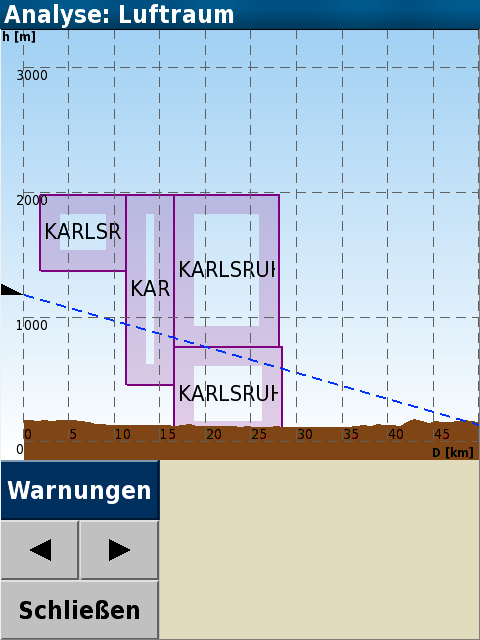
\includegraphics[angle=0,width=0.7\linewidth,keepaspectratio='true']{figures/analysis-airspace.png}
%\end{center}

Wenn man sich nahe eines Luftraumes befindet, wird diese Ansicht durch das
Luftraumwarnfenster unterbrochen.


\section{FLARM Luftverkehr, Erkennung und Darstellung}\index{FLARM!Erkennung}\index{FLARM!Darstellung}
Wenn \xc an ein \fl angeschlossen ist, ermöglicht \xc die Darstellung
des Luftverkehrs auf dem Display. Jedes erkannte Flugzeug, welches mit \fl
ausgestattet ist,  erscheint als kleines Dreieck in verschiedenen Farben  auf der Karte.

\achtung Benutze das \xc \fl- Radar nicht als Antikollosions-System, sondern halte die Augen auf und schaue
aus dem Flugzeug! Benutze eher die Warntöne des \fl , um nach sich nähernden Flugzeugen informiert zu werden!
Denke immer daran, daß es auch defekte \fl oder aber Flugzeuge ganz ohne \fl geben kann !!

Beachte, daß das \fl- Radar für eine normale Darstellung auf der Karte sehr unübersichtlich ist, es sei denn
Du befindest Dich im Kurbelmodus, wo das Radar auf die volle Bildschirmgröße gezoomt werden kann!
Beim Kurbeln oder bei Norden-Oben Darstellung ist die Kartendarstellung für die Erkennung des Luftverkehrs
kaum nützlich.

\subsection*{FLARM - Kartendarstellung}
Die \fl-Ziele sind als grüne, gelbe  oder rote kleine Dreiecke auf der Moving Map dargestellt.
\config{flarm-on-map}Die Spitzen der Dreiecke geben die Richtung an.

Im \fl-Radar werden die Ziele dagegen deutlich größer als Kreise mit innenliegenden,
richtungsangebenden Dreiecken  und bekommen je nach Gefahrensituation (Alarmlevel)
verschiedenen Farben.

\achtung Beachte unbedingt, daß die Ausrichtung je nach Kartendarstellung variiert!

Ist Nord-Oben eingestellt, so zeigen die Pfeile das absolute Bearing des Zieles.
Ist Kurs-Oben eingestellt, so zeigen die Pfeile in Richtung den relativen Kurs vom Ziel
zum eigenen Flugzeug.


%\begin{center}
%\includegraphics[angle=0,width=0.5\linewidth,keepaspectratio='true']{figures/flarmmap.png}
%\end{center}

Die Darstellung der Ziele auf dem \fl-Bildschirm kann durch Auswertung eines separaten
\sketch{figures/flarmmap.png}und individuell anpassbaren  \fl-Files Name, Kennzeichen etc.\ enthalten.
(Siehe hierzu~\ref{sec:flarm-ident-file} um Dich über Aufbau und Format des Files zu informieren)

Luftfahrzeuge im \fl-Stealth Modus oder die den Privat-Modus eingeschaltet haben können so jedoch nicht angezeigt werden.

\subsection*{FLARM Radar}
Um dieser Situation abzuhelfen, gibt es ein kleines Rechteck in der rechten unteren Kartenecke,
welches als Mini-\fl-Radar benutzt werden und entsprechend aktiviert vergrößert werden kann.

Die dargestellte Entfernung beträgt maximal 2000m. Im Hintergrund sind zwei hellgraue Kreise zu erkennen,
von denen der erste 1000m Durchmesser angibt, der zweite zeigt 2000m Durchmesser.
Flugzeuge, die sich jenseits 2000m Entfernung befinden, werden auf dem Kreis liegend dargestellt.

\marginpar{\includegraphics[angle=0,width=\linewidth,keepaspectratio='true']{figures/flarmrose.png}}

Alle \fl-Ziele werden gemäß des Alarmlevels  oder aber der Zugehörigkeit zum Team dargestellt:
\fl-Verkehr wird wie folgt eingefärbt:
\begin{itemize}
\definecolor{warning}{rgb}{1,0.64,0}
\definecolor{teammate}{rgb}{0.45,1,0}
\item \textcolor{black} {Keine Farbe für level 0, keine Aktion.}
\item \textcolor{warning} { Gelb für level 1, Warnung.}
\item \textcolor{red} {Rot für level 1 und 2, Alarm.}
\item \textcolor{teammate} {Grün für einen Team-Mitflieger.}
\item \textcolor{blue} {Blau dargestellt ist das angewählte Ziel.}
\end{itemize}


Jedes Ziel, dessen Alarmlevel größer als 1 ist, wird angezeigt.
Die angezeigte Höhe ist die absolute Höhe, gerundet auf 100m
\footnote{Je nach Einstellungen werden metrische oder englische Maße angezeigt..}.
Ein kleines Dreieck zeigt an, ob sich das Ziel über oder unter Dir befindet.
Im Beispiel zeigt das Radar das Ziel ungefähr 100m höher als Du selber.


Das \fl-Radar kann wieder ausgeschaltet werden, indem der Enter-Button gedrückt
wird -- auf dem \al  dient dazu der Drehknopf. Das \fl-Radar wird durch erneutes
Drücken bzw.\ drehen am Drehknopf wieder angeschaltet.

Werden neue \fl-Zeile erkannt, oder das \fl erzeugt eine Warnung, dann wird das
Radar automatisch wieder hochgefahren.

Um einen möglichst schnellen Überblick über mögliche Gefahren und deren
relativer Richtung zur Gefahr zu haben, wird, sowie der \fl-Alarmlevel des Zieles
eine Kollisionswarnung generiert, eine schwarze Linie vom Ziel zur Ecke des
Radars gezeichnet.


\subsection*{FLARM Radar -- Luftverkehr Anzeige / Dialog}
Wenn vom \fl Verkehr gemeldet wurde und das kleine \fl-Fenster geöffnet wurde, \config{flarmdisplay} so
kann durch doppelkicken des Fensters die \fl-Anzeige als Vollbildschirm dargestellt werden.

Es kann genausogut über

\begin{quote}
\bmenu{Info}\blink\bmenut{FLARM}{Radar}
\end{quote}

eingeschaltet werden.

Die Vollbildanzeige des \fl-Radars zeigt eine ganze Reihe von Details der erkannten Flugzeuge und -- je
nach Einstellungen im Konfigurationsmenü-- schließt sich das Fenster wieder von selber, wenn
kein Luftverkehr mehr erkannt wird.

\begin{center}
\includegraphics[angle=0,width=0.65\linewidth,keepaspectratio='true']{figures/dialog-flarm1.png}
\end{center}

In den vier Ecken des Radars sind folgende, zusätzliche Informationen angegeben:
\begin{description}
\item[Oben links]  Wenn vorhanden, die \fl-ID des Zieles.
\item[Oben rechts] Vario (Steigen/Sinken) des Zieles, errechnet aus der Höhenänderung,
\textsl{dementsprechend ungenau} und mit Vorsicht zu genießen\dots (Aktualisierungsfrequenz max.\ 1Hz)
\item[Unten links]  Entfernung zum Ziel.
\item[Unten rechts]  \textsl{Relative} Höhe zum Ziel.
\end{description}
\vspace{1em}

Auf diesem Bildschirm gibt es hier nur wenige Einstellmöglichkeiten, von oben nach unten:

\begin{description}
\item[~North up~]  Wenn angeklickt, wird der Radar-Bildschirm nach norden oben ausgerichtet.
Ansonten wird Kurs oben dargestellt.
\item[~A. Zoom~]   \gesture{runter-hoch} Der automatische Zoom versucht den Bildschirm derart darzustellen, daß die
Ziele optimal dargestellt werden.
Wenn nicht angeklickt, muß der Bildschirm manuell nachjustiert werden.
Die Hoch-Runter Geste aktiviert den Auto Zoom.
\item[~Avg/Alt~]  \gesture{rechts-links} Hiermit kann zwischen angezeigter Höhe und Vario der Zieles ausgewählt werden.
\item[~Details~]  \gesture{runter-rechts}  Mit dieser Auswahl erscheint ein separater
Dialog mit allen vorhandenen Details zum ausgewählten Ziel. Geste: Hoch-Runter.
\item[~+/-~ ] \gesture{hoch-runter} Manuelles ändern des Zoom - Bereiches von 500 Meter bis
zu 10000 Meter Reichweite.
\item[~$\triangleleft$/$\triangleright$~]  \gesture{links-rechts}  Auswahl des nächsten dargestellten Zieles.
Gestensteuerung mit Links/Rechts.
\end{description}

\begin{center}
\begin{tabular}{c c}
\includegraphics[angle=0,width=0.45\linewidth,keepaspectratio='true']{figures/cut-flarm2.png}&
\includegraphics[angle=0,width=0.45\linewidth,keepaspectratio='true']{figures/cut-flarm3.png}\\
\end{tabular}
\end{center}
Diese drei Bilder sind nacheinander aufgenommen und zeigen einen typischen Vorbeiflug zweier
mit \fl~ ausgestatteter Flugzeuge. Die Detaileinformationen sind farbig markiert wie oben bereits
beschrieben.

Vom ersten zum zweiten Photo sind ca.\ 15 Sekunden vergangen.
Das Steigen des blauen Zieles betrug $3,4m/s$ und hatte einen als nicht
kritisch zu betrachtenden Kurs bzgl. unseres Fliegers.

In der Zwischenzeit  ist die '' DC '' etwas mehr nach links abgedreht, wurde so als
eine mögliche Gefahr eingestuft und somit in rot dargestellt.
Das \fl-Radar schaltete den Zoom automatisch von 1000m auf 500m.

Im dritten Photo wird das kontinuierlich steigende Ziel in den Alarmlevel 1
eingestuft, gelb markiert und somit nicht länger als mögliche Gefahr
betrachtet und behandelt.


\section{Teamflug}\index{Teamflug}

Man kennt es: ''Wir fliegen heut' zusammen \dots'' und hat sich bereits 10Km vom
Startplatz entfernt in der diesigen Warmluftpampe voneinander getrennt. '' Wo zum Teufel steckst Du?''
''Unter einer Wolke'', ''rechts neben einer Burg, da wo die Windräder stehen'', '' bei der Autobahn'' etc\dots sind die üblichen
unbefriedigenden Antworten.


Das Teamflugsystem von \xc gestattet es, es einem Partner in \xc seine Position
\menulabel{\bmenut{Info}{2/3}\blink\bmenut{Team}{kode}}  in einem 5- stelligen Kode \textsl{exakt} mitzuteilen, ohne auf die Eingabe von Koordinaten und
  oder Bearings zurückgreifen zu müssen und ohne, daß es evtl. ''Konkurrenten'' eines Wettbewerbes mitbekommen
  (so sie denn den Referenzpunkt nicht kennen).

  Hierzu wird von beiden Piloten der gleiche  Referenzpunkt in \xc angegeben,
  dessen Richtung und Entfernung \xc intern in den Kode umrechnet.
  Anschließend haben beide Piloten die Entfernung und Bearing voneinander ''auf dem Schirm".

So kann  auch ohne Hilfe von  \fl, dessen Entfernungsmessungen und Empfangsstärke
mitunter oft stark schwanken  eine akkurate Bestimmung der jeweiligen Standorte vorgenommen werden.
Für die Zukunft wird aus o.g.\ Gründen an verschlüsselten Team Codes gearbeitet.

Um den Teamkode zu benutzen sollten alle Piloten eines Teams einen gemeinsamen Wegpunkt als Referenzpunkt
benutzen - 

\textsl{Sinnvollerweise sollten die Koordinaten  dieses Referenzpunkts \sketch{figures/dialog-teamcode.png}absolut identisch sein!!}.


Das heißt, alle Mitflieger eines Teams sollten identische Datenbanken benutzen.


Um TeamKode zu nutzen geht ihr wie folgt vor:
\begin{enumerate}
\item Mit \button{Setze WP} wird ein der Wegpunkt ausgewählt und anschließend bestätigt.
Es erscheint dann der eigene Kode, der dem Mitflieger übermittelt wird. 

\achtung \textsl{Es dauert ca.\ 2 Sekunden bis zur Aktualisierung - nicht zu schnell weiterklicken!}

Sinnvoll: 
Man einigt sich auf einen definitiven Punkt bereits vor dem Start und gleicht dessen Koordinaten ab\dots
\item Der Team-Kumpel macht exakt das gleiche.
\item Anschließend teilen beide sich Ihren fünfstelligen Kode gegenseitig über Funk mit
\item Mit \button{Kode Setzen} wird nun die Texteingabemaske aufgerufen und der empfangene Partner-Kode eingegeben.
\item Entfernung und Richtung des Kumpels erscheinen in den Feldern.
\end{enumerate}
Mit  \button{\fl Sperre} wird die \fl-Net-Datenbank aufgerufen.
Eine einfache  Tabelle  mit allen empfangenen Flugzeugen samt Wettbewerbs-ID und \fl-ID erscheint.
Hier kann schnell per Wettbewerbskennzeichen ein Teampartner ausgeblendet  werden.
Mit der Sperre wird dieser TeamPartner ''fixiert'' und während des fluges wenn wieder in Recichweite automatisch als Partner erkannt und dargestellt.

\textbf{Einschränkungen:}\\
Derzeit erlaubt  es \xc nur, \textsl{einen} Team Partner einzugeben, Ihr könnt aber über
das \fl-Radar mittels Team-Farben andere Team Mitglieder hinzufügen -- dies hat jedoch den Nachteil,
daß die Reichweite mitunter begrenzt ist. Dafür wird aktualisiert.
